\documentclass{article}

\title{Informe Bases de datos}
\date{April 2015}

\usepackage{graphicx}
\usepackage{caratula}
\usepackage{ulem}
\usepackage[spanish]{babel}
\usepackage[utf8]{inputenc}
\usepackage{listings}

\lstset{
	basicstyle=\footnotesize,
	breaklines=true,
	numbers=left,
	tabsize=2
}

\newcommand{\PK}[1]{\underline{#1}}
\newcommand{\FK}[1]{\dashuline{#1}}
\newcommand{\PKFK}[1]{\FK{\PK{#1}}}

\newcommand{\MR}[4]{
\noindent
\textbf{#1}(\PK{#2}, \FK{#3}, #4)\\
PK = CK = \{#2\}\\
FK = \{#3\}\\
}

\newcommand{\MRD}[4]{
\noindent
\textbf{#1}(\PKFK{#2}, \FK{#3}, #4)\\
PK = CK = \{#2\}\\
FK = \{#2, #3\}\\
}


\newcommand{\MRCK}[5]{
\noindent
\textbf{#1}(\PK{#2}, #3, \FK{#4}, #5)\\
PK = \{#2\}\\
CK = \{#2, #3\}\\
FK = \{#4\}\\
}
\begin{document}

\materia{Bases de datos}
\submateria{Primer Cuatrimestre de 2015}
\titulo{Trabajo Práctico 1}

\grupo{Grupo}
\integrante{Román Gorojovsky}{530/02}{rgorojovsky@gmail.com}

\begin{titlepage}
\maketitle
\thispagestyle{empty}
\end{titlepage} 

\tableofcontents

\section{Modelado del problema}
\subsection{Supuestos asumidos}
La dificultad principal en el diseño de este modelo provino de la tensión entre cierta tendencia de
los autores al diseño minimalístico que llevaba a soluciones incompletas; los conocimientos de los
autores, de cómo funciona realmente una elección lo que llevaba a complicar el problema a modelar;
la dificultad intrínseca del problema planteado y los espacios dejados por el enunciado a la
interpretación de los alumnos.

Decidimos incorporar un sólo elemento de la realidad no explícito en el enunciado: el hecho de que
los padrones cambian de elección a elección.  Esto complica un poco el diseño y modifica la
cardinalidad de algunas de las relaciones.

Menciono algunas de las ``realidades'' que se decidieron ignorar o simplificar: Las únicas
autoridades de mesa que \emph{deben} ser votantes de dicha mesa son los presidentes y
vicepresidentes.  Los fiscales tradicionalmente se ``agregan'' a la mesa en la que les corresponde
fiscalizar, y ni siquiera es obligatorio que voten en el mismo centro\footnotemark.  Por muchas
razones se podría argumentar que los técnicos no tendrían por qué trabajar sobre la mesa en la que
les corresponde votar, ni siquiera en su jurisdicción y otro tanto puede decirse de los responsables
de las camionetas.  El modelo soporta en principio estas libertades, siempre y cuando se cargue al
total de la población mayor a 16 años desde el arranque (para que todos los potenciales técnicos y
fiscales ``existan'', y asumiendo que ninguno es extranjero), no obstante lo cual, en la
construcción de los datos de ejemplo se exije a fiscales y técnicos que voten en su mesa.  No se
exijió nada sobre los responsables de las camionetas por simplificar la construción.

\footnotetext{Una resolución reciente cambió esto para CABA a partir de la última elección.}

Tampoco debería exijirse que los candidatos voten en el distrito a cuyo gobierno o representación se
presentan, la condición para ser candidato normalmente es haber nacido en el mismo o una cantidad de
años de residencia, generalmente 5 o 10.  De nuevo, si bien el modelo permite estas
``irregularidades'', se ha evitado a la hora de construír los datos de ejemplo.

Nada se dice en el enunciado sobre qué hacer con la fiscalización de las consultas populares.  Si
bien podría no ponerse ningún fiscal, se asignaron fiscales representando a partidos como si se
tratara de elecciones por cargos.

Una importante simplificación de la realidad es que se consideró a las elecciones legislativas
iguales a las ejecutivas: un candidato por partido, sin modelar listas de candidatos. Se asume
también que el total del padrón vota, es decir, el presentismo es del 100\%.


%% Seguro faltan, ya veré.

\subsection{DER}
En la figura 1 puede verse el diagrama de entidades y sus relaciones para la solución propuesta.

%% Posiblemente trate de imprimirlo en A3
\begin{figure}[h!]
	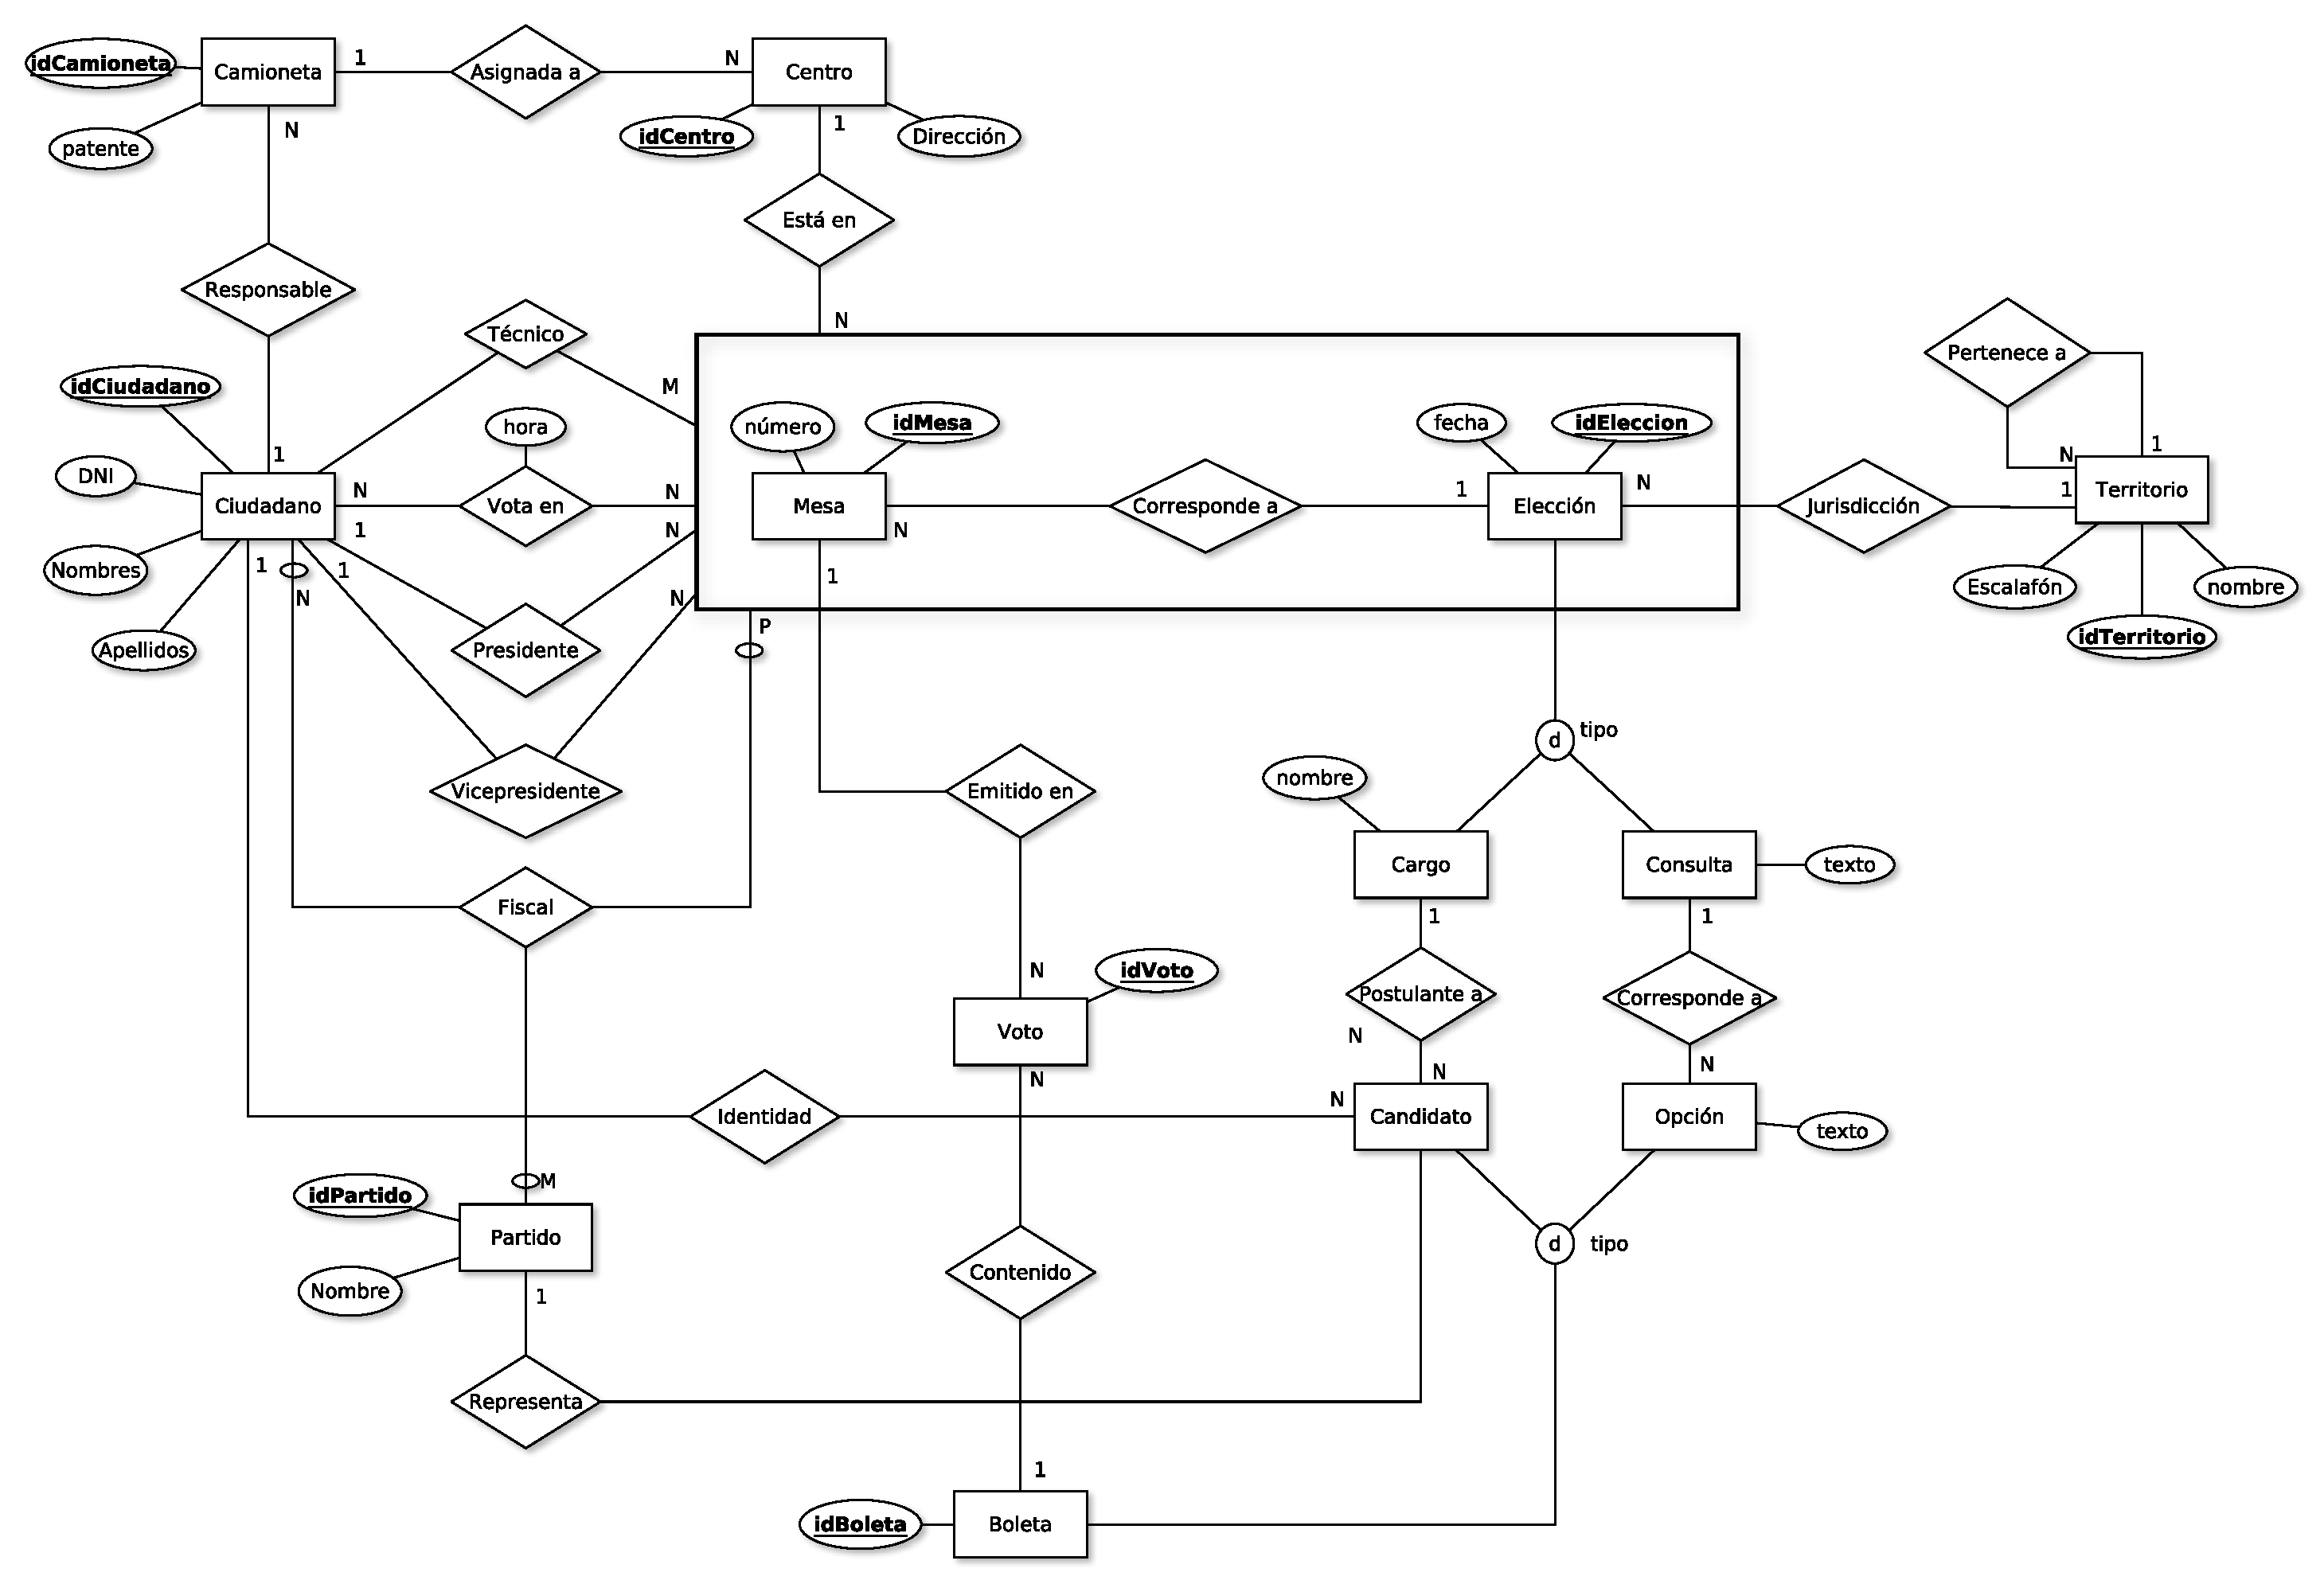
\includegraphics[scale=0.3]{DER}
    \caption{Diagrama Entidad-Relación}
\end{figure}

\subsection{Modelo Relacional}
Ese modelo resulta en el siguiente modelo relacional:\\

\MR{Boleta}{idBoleta}{idEleccion}{tipo}

\MRCK{Camioneta}{idCamioneta}{patente}{idCentro, idResponsable}{}

\MRD{Candidato}{idBoleta}{idCiudadano, idPartido, idEleccion}{}

\MRD{Cargo}{idEleccion}{}{titulo}

\MR{Centro}{idCentro}{}{direccion}

\MRCK{Ciudadano}{idCiudadano}{DNI}{}{nombres, apellidos, fechaNacimiento}

\MRD{Consulta}{idEleccion}{}{texto}

\MR{Eleccion}{idEleccion}{idJurisdiccion}{fecha, tipo}

\MR{Mesa}{idMesa}{idEleccion, idPresidente, idVicepresidente, idTecnico, idCentro}{numero}

\MRD{Opcion}{idBoleta}{idEleccion}{texto}

\MR{Partido}{idPartido}{}{nombre}

\MR{Territorio}{idTerritorio}{idPadre}{nombre, nivel}

\MR{Voto}{idVoto}{idBoleta, idMesa}{}

\noindent
\textbf{Fiscal}(\PKFK{idPartido, idCiudadano, idMesa})\\
PK = CK = \{(idPartido, idCiudadano, idMesa)\}\\
FK = \{idPartido, idCiudadano, idMesa\}\\

\noindent
\textbf{VotaEn}(\PKFK{idCiudadano, idMesa}, hora)\\
PK = CK = \{(idCiudadano, idMesa)\}\\
FK = \{idPartido, idCiudadano, idMesa\}

\pagebreak
Con las siguientes restricciones:\\

\noindent
\textbf{Boleta.idEleccion} debe estar en \textbf{Eleccion.idEleccion}.\\
\textbf{Boleta.idBoleta} debe estar o bien en \textbf{Candidato.idBoleta} o bien en
\textbf{Opcion.idBoleta}.

$\\$
\noindent
\textbf{Camioneta.idCentro} debe estar en \textbf{Centro.idCentro}.\\
\noindent
\textbf{Camioneta.idResponsable} debe estar en \textbf{Ciudadano.idCiudadano}.

$\\$
\noindent
\textbf{Candidato.idBoleta} debe estar en \textbf{Boleta.idBoleta}.\\
\noindent
\textbf{Candidato.idCiudadano} debe estar en \textbf{Ciudadano.idCiudadano}.\\
\noindent
\textbf{Candidato.idPartido} debe estar en \textbf{Partido.idPartido}.\\
\noindent
\textbf{Candidato.idEleccion} debe estar en \textbf{Eleccion.idEleccion}.

$\\$
\noindent
\textbf{Cargo.idEleccion} debe estar en \textbf{Eleccion.idEleccion}.

$\\$
\noindent
\textbf{Cargo.idEleccion} debe estar en \textbf{Eleccion.idEleccion}.

$\\$
\noindent
\textbf{Consulta.idEleccion} debe estar en \textbf{Eleccion.idEleccion}.

$\\$
\noindent
\textbf{Eleccion.idJurisdiccion} debe estar en \textbf{Territorio.idTerritorio}.\\
\textbf{Eleccion.idEleccion} debe estar o bien en \textbf{Cargo.idEleccion} o bien en
\textbf{Consulta.idEleccion}.

$\\$
\noindent
\textbf{Mesa.idEleccion} debe estar en \textbf{Eleccion.idEleccion}.\\
\textbf{Mesa.idPresidente}, \textbf{Mesa.idVicepresidente} y \textbf{Mesa.idTecnico} deben estar en
\textbf{Ciudadano.idCiudadano}.\\
\textbf{Mesa.idCentro} debe estar en \textbf{Centro.idCentro}.

$\\$
\noindent
\textbf{Opcion.idBoleta} debe estar en \textbf{Boleta.idBoleta}.\\
\textbf{Opcion.idEleccion} debe estar en \textbf{Eleccion.idEleccion}.

$\\$
\noindent
\textbf{Territorio.idPadre} debe estar en \textbf{Territorio.idTerritorio} y deben ser distintos.\\
\textbf{Territorio.idTerritorio} puede no estar en \textbf{Territorio.idPadre}.

$\\$
\noindent
\textbf{Voto.idBoleta} debe estar en \textbf{Boleta.idBoleta}.\\
\textbf{Voto.idMesa} debe estar en \textbf{Mesa.idMesa}.

$\\$
\noindent
\textbf{Fiscal.idPartido} debe estar en \textbf{Partido.idPartido}.\\
\textbf{Fiscal.idCiudadano} debe estar en \textbf{Ciudadano.idCiudadano}.\\
\textbf{Fiscal.idMesa} debe estar en \textbf{Mesa.idMesa}.\\
\textbf{Partido.idPartido} puede no estar en \textbf{Fiscal.idPartido}.\\
\textbf{Ciudadano.idCiudadano} puede no estar en \textbf{Fiscal.idCiudadano}.\\
\textbf{Mesa.idMesa} puede no estar en \textbf{Fiscal.idMesa}.\\

$\\$
\noindent
\textbf{VotaEn.idCiudadano} debe estar en \textbf{Ciudadano.idCiudadano}\\
\textbf{VotaEn.idMesa} debe estar en \textbf{Mesa.idMesa}

\subsection{Restricciones adicionales}
Sólo se puede ser autoridad de mesa de la mesa en la que se vota, es decir que para
\textbf{Mesa.idPresidente}y \textbf{Mesa.idVicepresidente} debe haber una entrada en \textbf{VotaEn}
tal que \textbf{VotaEn.idCiudadano} corresponde a uno de estos tres, y \textbf{VotaEn.idMesa} a la
mesa en cuestión.




\section{Implementacion}
El trabajo se implementó en una base \emph{MySql} 5, 5.6 para ser precisos, y fue posible traducir
el modelo relacional directamente a la base de datos definitiva.  Se usaron enteros para todos los
atributos que se pudieron representar con ellos (en particular y por simplicidad, la patente de las
camionetas se representó como enteros de 6 cifras), para las fechas se usaron \texttt{datetimes} y
para las demás, \texttt{varchar} con tamaños entre arbitrarios y elegidos por experiencia anterior.

\subsection{Stored Procedures}
Para resolver las tres funcionalidades pedidas se utilizaron los siguientes Stored Procedures:

% Acá irá el código lisa y llanamente
\lstinputlisting[language=SQL, firstline=5, lastline=91]{../generadores/add_stored_procedures.sql}

\section{Datos de testing}
\subsection{Scripts de carga de datos}



\end{document}
